\section{进程状态控制}

\subsection{基本概念}

在操作系统课程的学习中我们知道 ,进程其实是一个“执行中的程序”。程序是一个没有生
命的实体 ,只有 在操作系统执行静态的、放在磁盘中的代码段时 ,它才能成为一个活动
的实体 ,我们称其为进程。

在运行过程中 ,进程是一个实体。每一个进程都有它自己的地址空间 ,一般情况下 ,包
括文本区域  (text  region)  、数据区域  (data region)  和堆栈  (stack
 region)  。文本区域存储处理器执行的代码 ;数据区域 存储变量和进程执行期间使用
的动态分配的内存 ;堆栈区域存储着活动过程调用的指令和本地变量。
\begin{figure}[H]
	\centering
	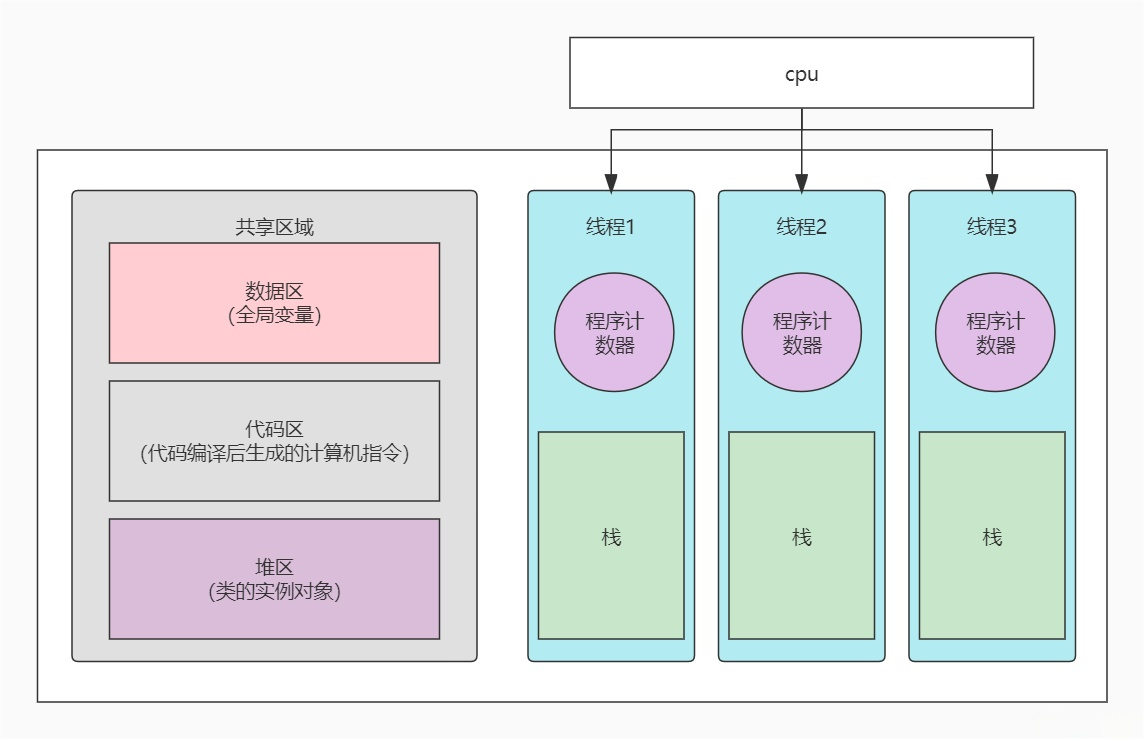
\includegraphics[width=14cm,height=8cm]{figures/05-02-01-进程的数据结构.png}
	\caption{进程的数据结构}
\end{figure}  

进程的创建、销毁与切换存在着较大的时空开销,一种轻型的进程技术线程用来减少开销。
线程被设计成进程的一个执行路径,同一个进程中的线程共享进程的资源,因此系统对线
程的调度所需的成本远远小于进程。

\begin{figure}[H]
	\centering
	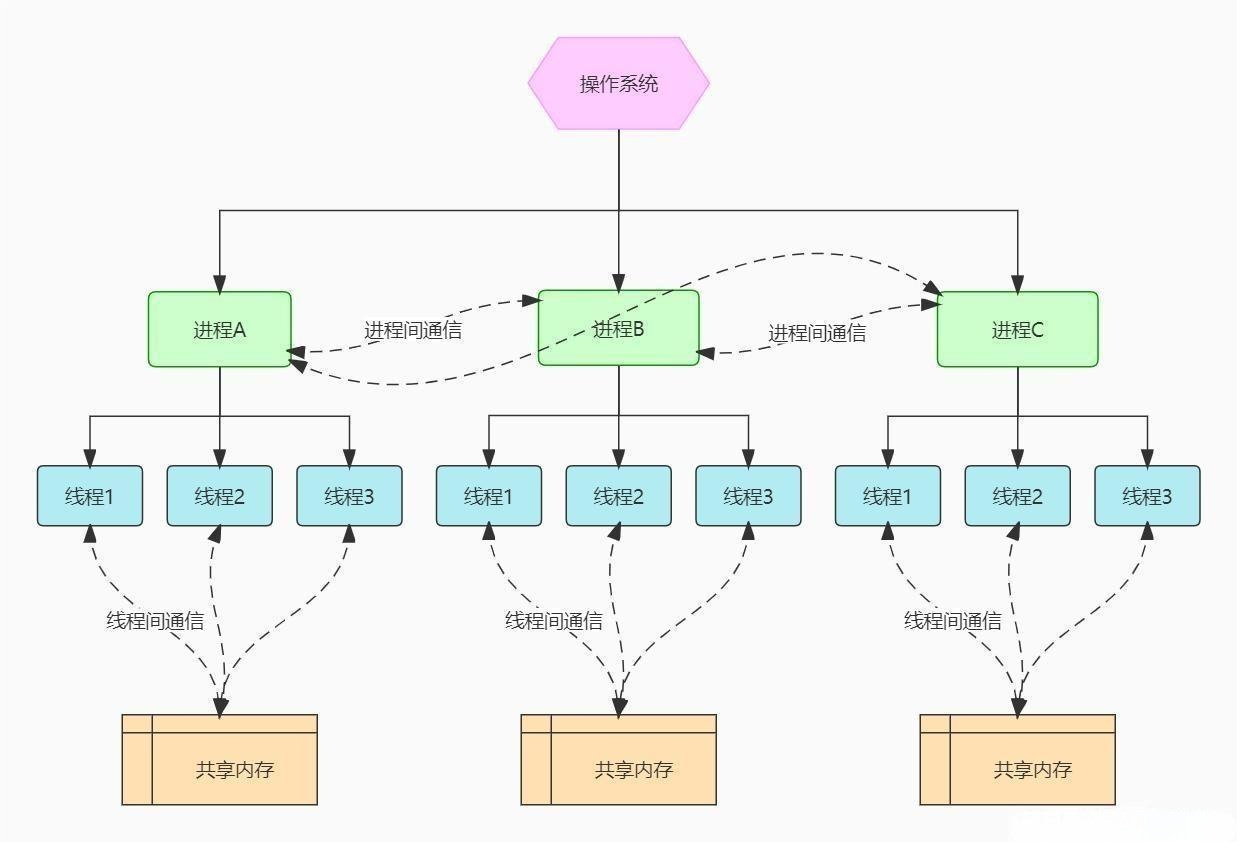
\includegraphics[width=14cm,height=11cm]{figures/05-02-01-线程与进程间的关系.png}
	\caption{线程与进程间的关系}
\end{figure}  

在 NPUcore 中 ,我们使用 TCB结构体来描述一个进程 ,该结构体可以完整地描述一
个进程的内容和结构。 利用该结构体 ,我们可以像 linux
 一样使用进程来模拟线程。这与windows操作系统的设计思路是不同的,其线程的实现依
 靠单独的一套 thread\_control\_block 完成。
 
因此线程在 NPUcore 中的理解变为了这样——一个可以与同线程组( tg1d 共享内存空间
的进程即为线程。

NPUCore进程管理的代码树如下:
\begin{lstlisting}[language=Rust]
	os
	|--src
	|--task
	|--context.rs //存储上下文信息
	|--elf.rs //ELF文件加载和解析
	|--manager.rs //任务管理器的结构存储
	|--mod.rs//任务操作系统任务管理和调度的实现
	|--pid.rs//实现内核栈、进程分配器、内核栈分配器等数据结构及操作
	|--processor.rs // 进程轮询的主体和processor的声明与实现
	|--signal.rs //
	|--switch.rs //调用switch汇编函数的接口,实现任务上下文切换
	|--switch.S //任务上下文切换的汇编实现
	|--threads.rs//实现用户空间多线程快速互斥锁(Futex)
	|--task.rs //涉及TCB模块的声明以及方法的实现,以及rusage信号量的声明。
\end{lstlisting}

\subsection{进程管理重要数据结构}
\subsubsection{进程标识符\ PidHandle}
同一时间存在的所有进程都有一个唯一的进程标识符,将其抽象为 PidHandle 类型。
\begin{lstlisting}[language=Rust]
	//os/src/task/pid.rs
	pub struct PidHandle(pub usize);
\end{lstlisting}

进程标识符是一个64位的无符号整数 ,用来标识进程ID。进程标识符的分配和回收由标
识符分配 器 RecycleAllocator 完成。我们一般简称其为 PID。

\subsubsection{内核栈\ KernelStack}
内核在创建进程的时候 ,在创建task\_struct的同时 ,会为进程创建两个栈 ,第一个
栈也就是上面分析到的 进程用户栈 ,存在于用户空间使用 ,另外还有一个内核栈 ,存
放在内核空间。

\textbf{内核栈存在的意义 :}如系统调用在陷入内核后 ,系统调用中也是存在函数调
用和自动变量 ,这些都需 要栈支持。

\textbf{每个进程都要有独自的内核栈的必要性:}所有进程在运行时 ,都有可能通过系
统调用陷入内核态继续 执行 ,假设第一个进程陷入内核执行的时候,需要等待某个资
源,主动schedule() ,让出CPU ,第二个进 程假设也通过系统调用进入了内核态 ,
如果进程共享内核栈 ,那么第二个进程在系统调用压栈时会破坏第一个进程栈数据。

每个应用都有自己的内核栈 ,因此 KernelStack 的内部就是其所属进程的 PID 号。

\begin{lstlisting}[language=Rust]
	//os/src/task/pid.rs
	pub struct KernelStack(pub usize);
\end{lstlisting}

它提供了以下方法 :

1.返回当前内核栈在内核空间中的栈顶和栈底位置 :
\begin{lstlisting}[language=Rust]
	pub fn kernel_stack_position(kstack_id:usize) -> (usize,usize) {
		let top = TRAMPOLINE - kstack_id * (KERNEL_STACK_SIZE + PAGE_SIZE);
		let bottom = top - KERNEL_STACK_SIZE;
		(bottom, top)
	}
\end{lstlisting}

2.内核栈分配器 :
\begin{lstlisting}[language=Rust]
	pub fn kstack_alloc() -> KernelStack {
		let kstack_id = KSTACK_ALLOCATOR.lock().alloc();
		let (kstack_bottom, kstack_top) = kernel_stack_position(kstack_id);
		KERNEL_SPACE.lock().insert_framed_area(
		kstack_bottom.into(),
		kstack_top.into(),
		MapPermission::R|MapPermission::W,);
		KernelStack(kstack_id)
	}
\end{lstlisting}

该分配器先从全局实例化的 KSTACK\_ALLOCATOR 中获取内核栈编号。它调用了  kernel\_stack\_position
函数来根据进程标识符计算内核栈在内核地址空间中的位置 ,随即将一个逻辑段插入
内核地址空间 KERNEL\_SPACE 中  (详情见内存管理章节)。

3.将内核栈从内核空间中移除 :
\begin{lstlisting}[language=Rust]
	impl Drop for KernelStack {
		fn drop(&mut self) {
			let (kernel_stack_bottom, _) = kernel_stack_position(self.0);
			let kernel_stack_bottom_va:VirtAddr = kernel_stack_bottom .into();
			KERNEL_SPACE
			.lock()
			.remove_area_with_start_vpn(kernel_stack_bottom_va.into())
			.unwrap();
			KSTACK_ALLOCATOR.lock().dealloc(self.0)
		}
	}
\end{lstlisting}

4.push\_on\_top 方法 :
\begin{lstlisting}[language=Rust]
	impl KernelStack{
		#[allow(unused)]
		pub fn push_on_top<T>(&self,value:T) -> *mut T
		where
		T:Sized,
		{
			let kernel_stack_top = self.get_top();
			let ptr_mut = (kernel_stack_top - core::mem::size_of::<T>()) as *mut T;
			unsafe {
				*ptr_mut = value;
			}
			ptr_mut
		}
		pub fn get_top(&self) -> usize {
			let (_,kernel_stack_top) = kernel_stack_position(self.0);
			kernel_stack_top
		}
	}
\end{lstlisting}

该方法可以将一个类型为  T 的变量压入内核栈顶并返回其裸指针 ,这也是一个泛型函数。  它在实现的时 候用到了  get\_top 方法来获取当
前内核栈顶在内核地址空间中的地址。

\subsubsection{进程控制块\ PCB}
为了使并发执行的程序独立运行 ,描述进程的基本情况和活动过程 ,进而管理和
控制进程 ,操作系统专门 配置了一个数据结构——进程控制块。在 NPUcore 中 ,我们使用 TCB 这一名字代替 PCB 来同时用作进程控制块和线程控制块。但是在
本章中 ,为了简化逻辑 ,我们尽量只讨论单线程的情况 ,也就是仅仅 把 TCB 看
作是进程控制块。

TCB作为进程实体的一部分 ,记录了操作系统所需的 ,描述进程的当前情况以及管理
进程运行的全部信息,是操作系统中最重要的数据结构。整个进程管理模块,
正是围绕着TCB数据结构的生命周期来展开,通过控制TCB模块的生命周期来实
现进程的创建,调度和回收。

\textbf{作为独立运行基本单位的标志 :}当一个程序  (含数据)  配置了TCB后 ,
就标志着它已经是一个能在多道程序环境下独立运行、合法的基本单位。系统是通过
TCB感知进程的存在的 ,TCB已成为进程存在 于系统 的唯一标志。

\textbf{能实现间断性运行方式 :}当进程因阻塞而暂停运行时 ,他必须保留运行时
的CPU现场信息 ,再次被调度运行时 ,还需要恢复运行时的CPU现场信息。在有了
TCB后 ,系统将CPU现场信息保存在被中断进 程的TCB中 ,供该进程再次被调度时恢复其CPU现场信息 。  由此可知 
,在多道程序环境下 ,传统意义 上的程序无法保护自身运行环境 ,
无法保证其执行结果的可再现性 ,失去运行意义。

\textbf{提供进程管理所需的信息 :}当调度某进程运行时 ,只能根据该进程TCB
只能记录的程序和数据的始址指针 ,来找到相应的程序和数据 ;在进程运行期间 ,  
当需要访问文件系统中的文件或I/O设备时 ,也需 要借助TCB中的信息。可见 ,
在进程的生命周期中 ,操作系统总是根据TCB中的信息来控制和管理进 程。

\textbf{提供进程调度所需的信息 :}只有处于就绪状态的进程才能被调度执行 ,
而TCB就提供了该进程处于何种状态的信息。

\textbf{实现与其他进程的同步和通信}

在NPUcore中 ,任务控制块 TCB(Task Control Block) 将直接作为 PCB 进行使用。
下图是NPUcore中进 程控制块的具体组成。

\begin{figure}[H]
	\centering
	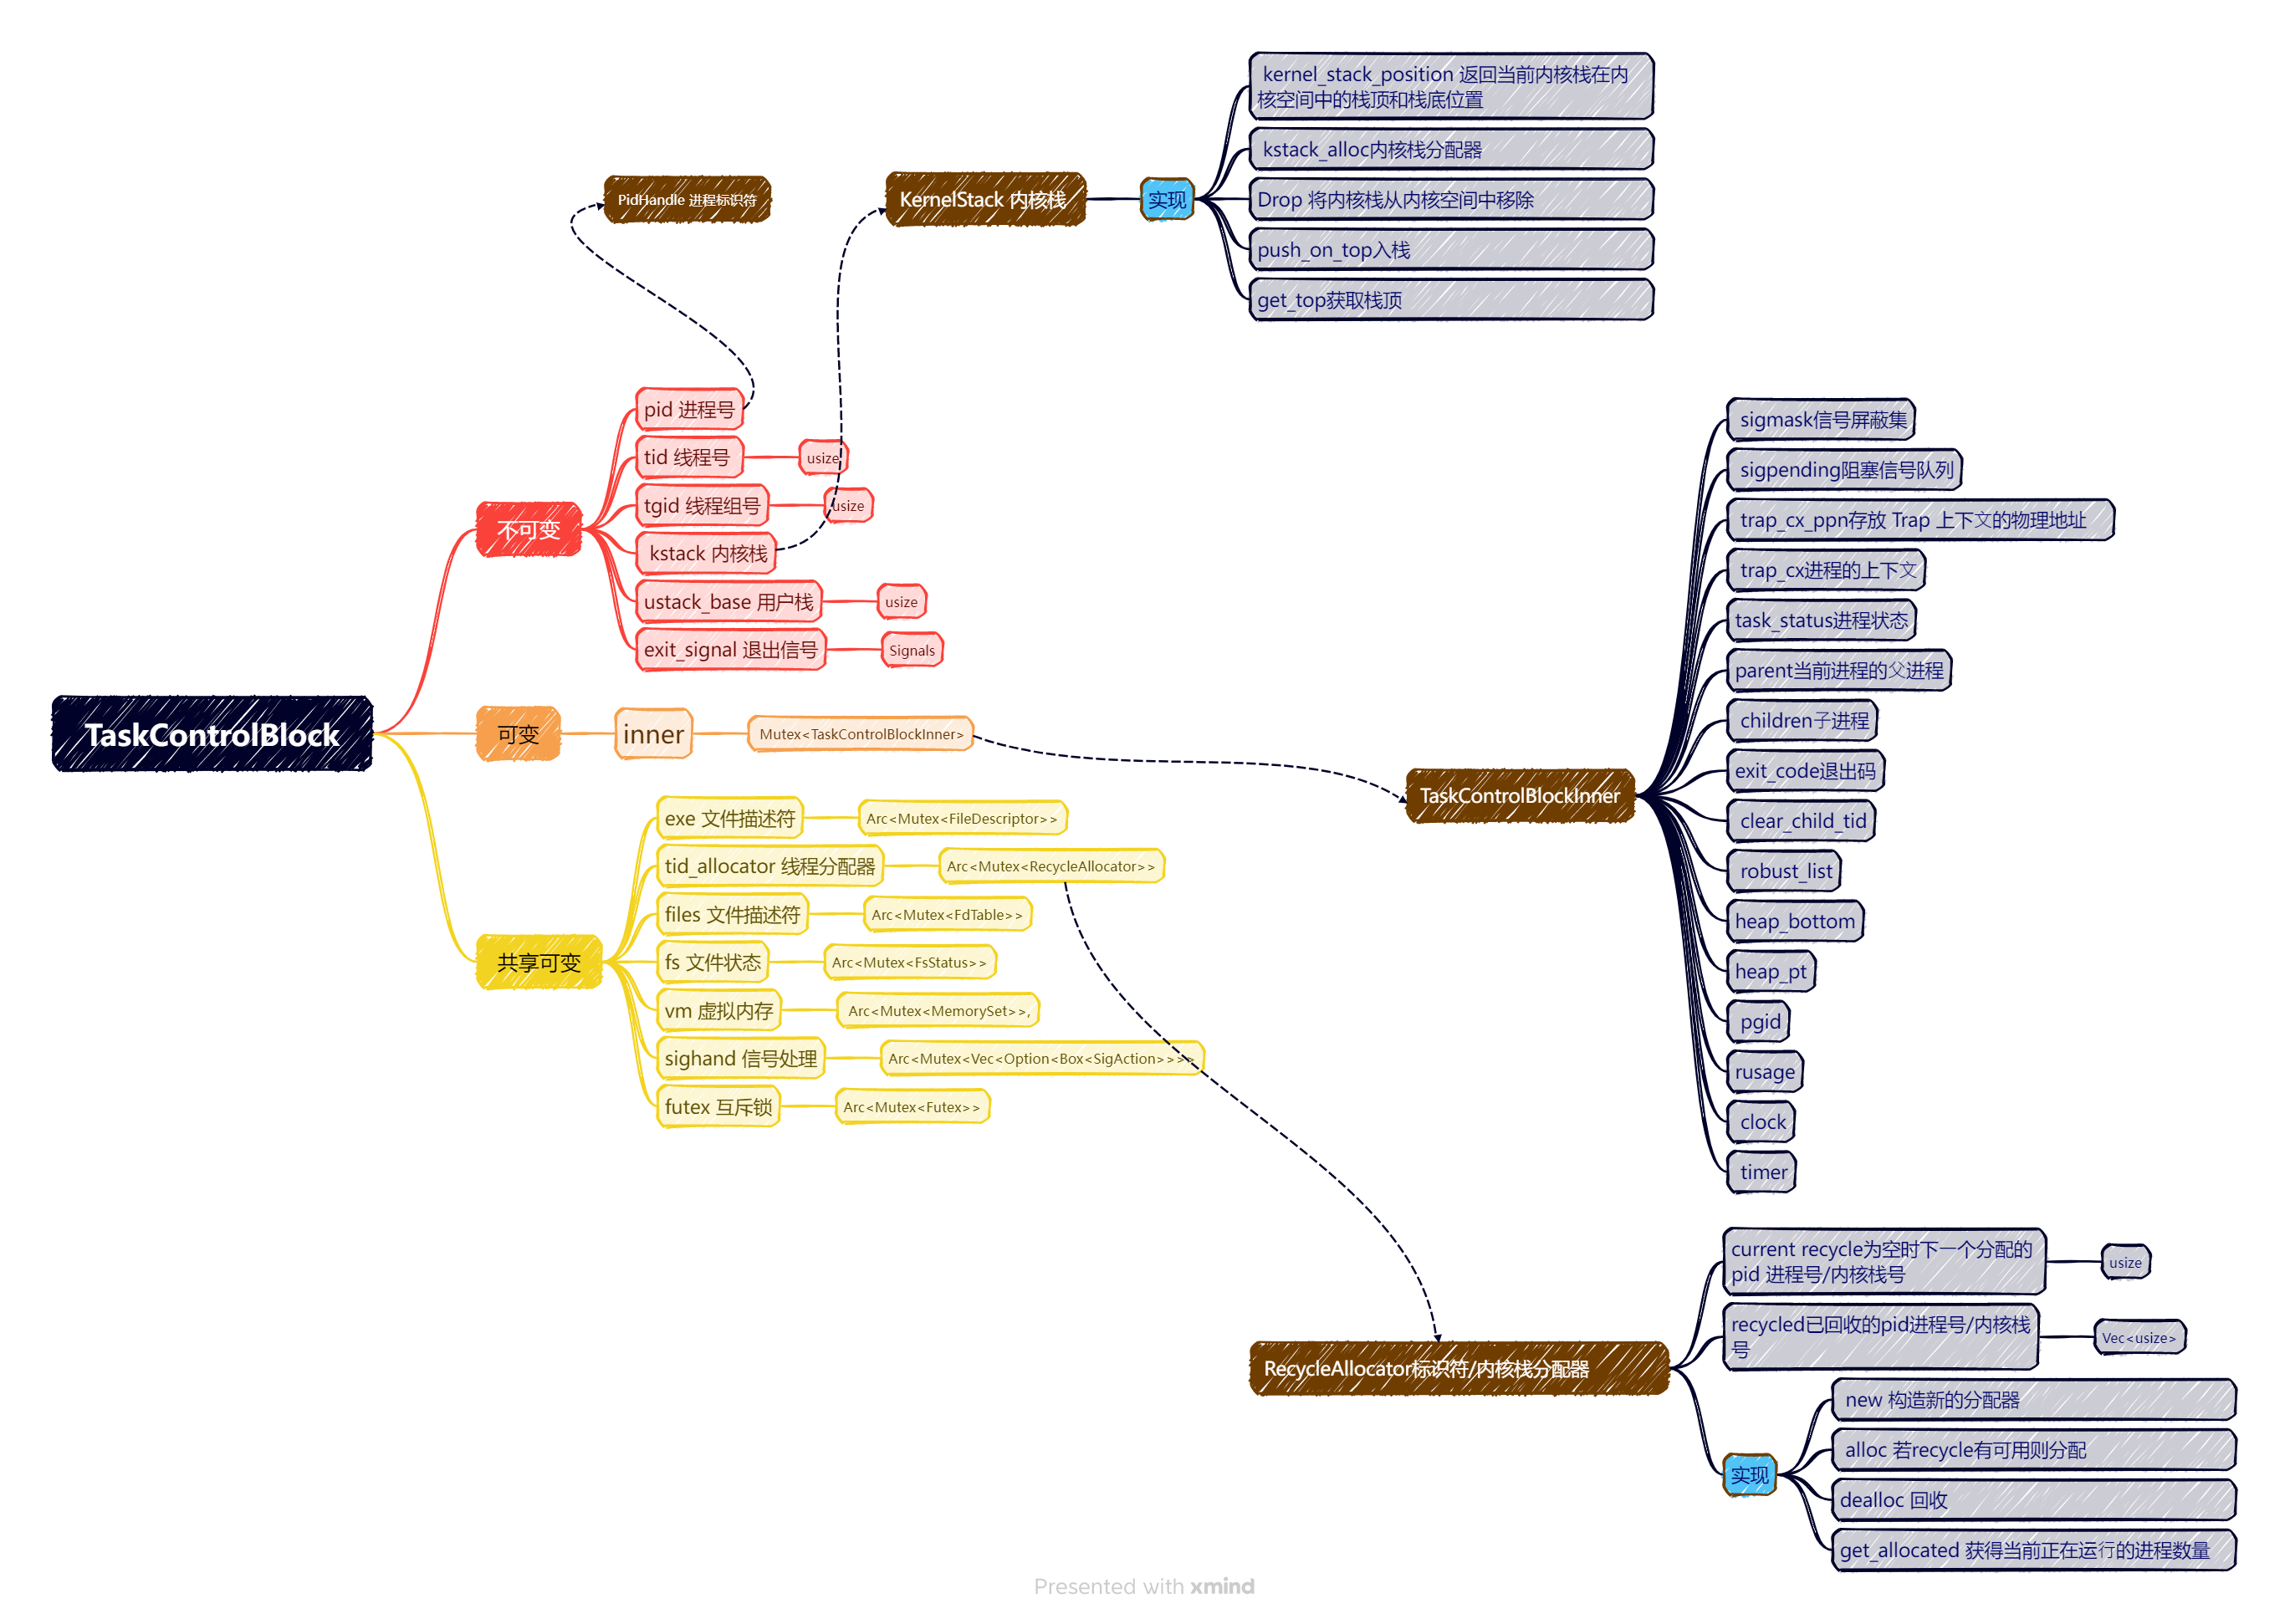
\includegraphics[width=14cm,height=11cm]{figures/05-02-01-NPUcore中进程控制块的具体组成.png}
	\caption{NPUcore中进程控制块的具体组成}
\end{figure}    

由于该数据结构的成员过多 ,且很多成员变量都是与信号及多线程的锁相关的 ,因此这
里只挑选部分成员 变量进行讲解。

\begin{lstlisting}[language=Rust]
	//os/src/task/task.rs
	pub struct TaskControlBlock {
		// immutable
		pub pid:PidHandle,
		pub tid:usize,
		pub tgid:usize,
		pub kstack:KernelStack,
		pub ustack_base:usize,
		pub exit_signal:Signals,
		// mutable
		inner:Mutex<TaskControlBlockInner>,
		// shareable and mutable
		pub exe:Arc<Mutex<FileDescriptor>>,
		pub tid_allocator:Arc<Mutex<RecycleAllocator>>,
		pub files:Arc<Mutex<FdTable>>,
		pub fs:Arc<Mutex<FsStatus>>,
		pub vm:Arc<Mutex<MemorySet>>,
		pub sighand:Arc<Mutex<Vec<Option<Box<SigAction>>>>>,
		pub futex:Arc<Mutex<Futex>>,
	}
	pub struct TaskControlBlockInner {
		pub sigmask:Signals,
		pub sigpending:Signals,
		pub trap_cx_ppn:PhysPageNum,
		pub task_cx:TaskContext,
		pub task_status:TaskStatus,
		pub parent:Option<Weak<TaskControlBlock>>,
		pub children:Vec<Arc<TaskControlBlock>>,
		pub exit_code:u32,
		pub clear_child_tid:usize,
		pub robust_list:RobustList,
		pub heap_bottom:usize,
		pub heap_pt:usize,
		pub pgid:usize,
		pub rusage:Rusage,
		pub clock:ProcClock,
		pub timer:[ITimerVal;3],
	}
\end{lstlisting}

TCB 由可变部分、不可变部分及可共享且可变部分组成。

1.不可变部分 :

( 1) pid :进程号在进程创建后就是唯一的身份标识 ,所以肯定不变。  
它的类型是 PidHandle 	

(2)   kstack :这是每个应用的内核栈。

(3)  ustack base: 用户栈的基地址 

(4)  exit signal: 退出信号

2.可变部分:inner : Mutex<TaskControlBlockInner>

TaskControlBlockInner 结构体的定义如下 :

\begin{lstlisting}[language=Rust]
	pub struct TaskControlBlockInner {
		pub sigmask:Signals,
		pub sigpending:Signals,
		pub trap_cx_ppn:PhysPageNum,
		pub task_cx:TaskContext,
		pub task_status:TaskStatus,
		pub parent:Option<Weak<TaskControlBlock>>,
		pub children:Vec<Arc<TaskControlBlock>>,
		pub exit_code:u32,
		pub clear_child_tid:usize,
		pub robust_list:RobustList,
		pub heap_bottom:usize,
		pub heap_pt:usize,
		pub pgid:usize,
		pub rusage:Rusage,
		pub clock:ProcClock,
		pub timer:[ITimerVal;3],
	}
\end{lstlisting}	

同上 ,我们也不介绍信号与锁相关的成员变量。

trap\_cx\_ppn :这个东西的作用是把存放 Trap 上下文的物理地址拿出
来 ,从而便于使用

\begin{lstlisting}[language=Rust]
	let trap_cx_ppn = memory_set
	.translate(VirtAddr::from(TRAP_CONTEXT).into())
	.unwrap()
	.ppn();
\end{lstlisting}	
	
	task\_cx:类型是 TaskContext是进程的上下文

\begin{lstlisting}[language=Rust]
	pub struct TaskContext {
		/// return address (e.g.__restore ) of__switch ASM function
		ra:usize,
		/// kernel stack pointer of app
		sp:usize,
		/// s0-11 register, callee saved
		s:[usize; 12],
	}
\end{lstlisting}

TaskManager:进程管理模块,维护两个循环队列,一个是就绪态队列,一个是阻
塞态任务队列,队列中的内容都是TCB模块的指针。
\begin{lstlisting}[language=Rust]
	pub struct TaskManager {
		pub ready_queue:
		VecDeque<Arc<TaskControlBlock>>,
		pub interruptible_queue:
		VecDeque<Arc<TaskControlBlock>>,
	}
\end{lstlisting}
ready\_queue:就绪态队列

interruptible\_queue:阻塞态任务队列

Processor:用于保存当前任务的arc指针和空闲的任务上下文(用于进程切换)。
\begin{lstlisting}[language=Rust]
	pub struct Processor {
	current:Option<Arc<TaskControlBlock>>,
	idle_task_cx:TaskContext,
}
\end{lstlisting}
current 表示在当前处理器上正在执行的任务
\
idle\_task\_cx 表示当前处理器上的 idle 控制流的任务上下文

TaskStatus:基本的任务状态枚举,包括就绪态,运行态,僵尸态(等待回
收),阻塞态(等待激活以进入就绪态)。
\begin{lstlisting}[language=Rust]
	pub enum TaskStatus {
	Ready,
	Running,
	Zombie,
	Interruptible,
}
\end{lstlisting}

说明进程有四种状态 :就绪 、正在运行、“僵尸”状态  (表示该进程即将被回收)  
以及可中断状态。

parent 是 TCB 的一个弱引用 ,他表示当前进程的父进程 ,同理 children 表示子进程exit\_code , 当进程调用  exit 系统调用主动退出或者执行出错由
内核终止的时候 ,它的退出码exit\_code 会被内核保存在它的任务控制块中 ,
并等待它的父进程通过  waitpid 回收它的资源的同时也 收集它的 PID 以及退出码。

\subsubsection{标识符/内核分配器\ RecycleAllocator}
对于进程标识符和内核栈,NPUCore都使用 RecycleAllocator 分配器来分配和回收。
\begin{lstlisting}[language=Rust]
	//os/src/task/pid.rs
	pub struct RecycleAllocator {
		current:usize,
		recycled:Vec<usize>,
	}
\end{lstlisting}

current 为若 recycled 数组为空时下⼀个分配的 pid 进程号/内核栈号 ,
每次分配后都会+1 ; recycled 数组保存了当前已回收的 pid 进程号/内核栈号。

该分配器实现了以下四个方法 :

\begin{lstlisting}[language=Rust]
	impl RecycleAllocator {
		pub fn new() -> Self {
			RecycleAllocator {
				current:0,
				recycled:Vec::new(),
			}
		}
		pub fn alloc(&mut self) -> usize {
			if let Some(id) = self.recycled .pop() {
				id
			} else {
				self.current += 1;
				self.current - 1
			}
		}
		pub fn dealloc(&mut self,id:usize) {
			assert!(id<self.current);
			assert!(
			!self.recycled.iter().any(|i|*i == id),
			"id {} has been deallocated!",
			id
			);
			self.recycled.push(id);
		}
		pub fn get_allocated(&self) -> usize {
			self.current - self.recycled.len()
		}
	\end{lstlisting}
	
	\textbf{new() :}构造方法 。只会在第⼀次实例化时调用。
	
\textbf{	alloc(\&mut self) :}分配器。若 recycled 数组中有可使用的
	 pid 号/内核栈号 ,则直接分配 ,否则 生成⼀个新的 pid 号。
	
	\textbf{dealloc(\&mut self, id: usize):}回收器。需要检查合法性才会回收。
	
\textbf{	get\_allocated(\&self) :}获得当前正在运行的进程数量。
	
	有了分配器后 ,我们可以将进程分配器分别实例化,
	
	实例化进程标识符分配器和内核栈分配器:
	\begin{lstlisting}[language=Rust]
		lazy_static!{
			static ref PID_ALLOCATOR:Mutex<RecycleAllocator> = Mutex: :new(RecycleAllocator::new()
			static ref KSTACK_ALLOCATOR:Mutex<RecycleAllocator> = Mutex: :new(RecycleAllocator::new()
		}
	\end{lstlisting}
	
	注意 ,这里的结构体 RecycleAllocator 并不仅仅是 PID 分配器 ,
	还可以做内核栈分配器。 
	
	分配器将会分配出去一个 PidHandle ,将其包装为一个全局分配进程标识符
	的接口 pid\_alloc 提供给内核的其他子模块,并为 PidHandle 实现 
	Drop Trait 来允许编译器进行自动的资源回收:
	
	\begin{lstlisting}[language=Rust]
		pub fn pid_alloc() -> PidHandle {
			PidHandle(PID_ALLOCATOR.lock().alloc())
		}
		impl Drop for PidHandle {
			fn drop(&mut self) {
				PID_ALLOCATOR.lock().dealloc(self.0);
			}
		}
	\end{lstlisting}
	
